\scanpage{16}
\mspage{\unsure{3|5})}
\textcircled{3} Soit
\deleted{$X\supset Y$, $X$ \unsure{muni de sous-espaces}}
\inserted{$T$ un vois. \deleted{tub.} conique absolu de $Y$.}
% P03: the epsilon-like lowered group is overworked; no independent strike establishes its cancellation state.
\unsure{Soient|Soit} $\unsure{T'_\varepsilon|T'\deleted{_\varepsilon}}\subset T$.
On dit que $T'$ est \uline{sous-espace cônique} dans $T$ si on a
\[
(12)\qquad\left\{\begin{array}{ll}
a)&T'\text{ stable par homothéties }\lambda\in\mathbf{I}\qquad
\deleted{\unsure{\lambda T'\subset T'}}\\
% P04: the initial P has a small raised/retraced remnant, without a recoverable earlier token.
b)&\text{\unsure{Pour} cette opération, }T'\text{ est un voisinage}
\end{array}\right.
\]
\deleted{tubulaire} cônique de $Y$.
\uline{NB} On aura nécessairement $\unsure{\dot T'}=T'\cap\dot T$,
$T'_\lambda=T'\cap T_\lambda$ ;
\deleted{Si $(T_i)_{i\in I}$ est une famille\unsure{,}}
\inserted{la donnée de $T'$ équivaut à}
celle d'un sous-espace fermé $\dot T'$ de $\dot T$
et d'un sous-espace $\unsure{T'|Y'}$ de $Y$, tel que $Y'\supset0.\dot T'$, et,
on a
\[
% P08: separate unrecoverable raised mark above the double-stem I; no established accent meaning or cancellation state.
T'=\operatorname{Im}(\overset{\unsure{}}{\mathbb{I}}\times
\dot T'\unsure{\lambda|\deleted{\lambda}|\ell|\}}
\unsure{\mathrel{\relbar\joinrel\relbar}|\longrightarrow}T)\cup Y'.
\]
\margin{On dit que $T'$ est cônique \uline{strict}
si $T'\cap Y=0.\dot T'$
--- ces $T'$ correspondent donc aux fermés
$\dot T'$ de $\dot T$.}

On dira qu'une structure cônique sur
un $T\supset Y$ est \uline{compatible} avec des sous-espaces
\inserted{fermés} $T_i$ de $T$ $(i\in I)$ si ces derniers
sont côniques pour cette structure.

Soit $T$ un voisinage conique de $Y\subset X$
dans $X$, soit $X'$ \unsure{p}artie fermée de $X$. On
% P11/P12: the apparent mark above the end of compatible belongs to the hooked descender of fermée.
dit que $T$ est \uline{compatible} avec $X'$ si
$X'\cap T$ est cônique dans $T$. On dit qu'il
est \uline{strictement compatible}$^{*}$ avec $T$, si
$T$ est voisinage conique strict, et s'il existe
un voisinage cylindrique de $\dot T$ dans
$X^*=X\setminus\mathring T$, compatible avec
$X'{}^{\unsure{*|\mathrm r}}=X'\cap X^*$,
ou ce qui revient au $=$, s'il existe un
voisinage $E$ de $\dot T$ dans $X^*$, et un iso
\margin{\deleted{\unsure{Définir la notion pour $X'$|dire \illegible{1} compatible avec $X'$}}}
\margin{$^{*}$ \deleted{\uline{\unsure{aussi dire|transversal}} \uline{\unsure{strict}}}}
\margin{modifier \unsure{sans doute} la définition des
voisinages côniques \unsure{strict|stricts}\ldots}
% P18: one unheaded separator/leader beside the lower marginal note, leaning slightly right down the original page.
\margin{\figure{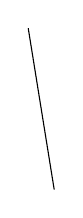
\begin{tikzpicture}[x=1cm,y=1cm]
\draw (0,0)--(0.33,-2.05);
\end{tikzpicture}}}
\margin{15}
